% Source: graduate-coursework/Sp26/CSCE775/course_notes/ch5_exercises/exercise_5_1.tex

\documentclass[border=4pt]{standalone}
\usepackage{amsmath, amssymb}
\usepackage{graphicx}
\usepackage{tikz}
\usepackage{xcolor}
\usetikzlibrary{positioning}

\definecolor{garnet}{HTML}{73000A}
\definecolor{black90}{HTML}{363636}
\definecolor{atlantic}{HTML}{466A9F}

\begin{document}
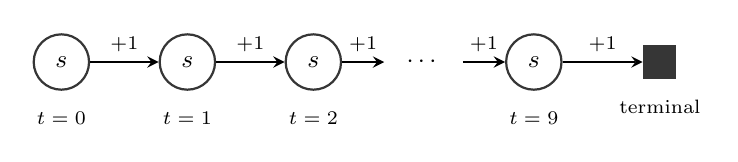
\begin{tikzpicture}[
    state/.style={circle, draw=black90, thick, minimum size=20pt, inner sep=0pt, font=\small},
    terminal/.style={rectangle, fill=black90, minimum size=12pt, inner sep=0pt},
    every node/.style={font=\small},
    >=stealth
]
    \node[state] (s0) at (0,0) {$s$};
    \node[state] (s1) at (1.6,0) {$s$};
    \node[state] (s2) at (3.2,0) {$s$};
    \node at (4.6,0) {$\cdots$};
    \node[state] (s9) at (6.0,0) {$s$};
    \node[terminal] (T) at (7.6,0) {};

    \draw[->, thick] (s0) -- node[above]{\scriptsize $+1$} (s1);
    \draw[->, thick] (s1) -- node[above]{\scriptsize $+1$} (s2);
    \draw[->, thick] (s2) -- node[above]{\scriptsize $+1$} (4.1,0);
    \draw[->, thick] (5.1,0) -- node[above]{\scriptsize $+1$} (s9);
    \draw[->, thick] (s9) -- node[above]{\scriptsize $+1$} (T);

    \node[below=4pt of s0] {\scriptsize $t=0$};
    \node[below=4pt of s1] {\scriptsize $t=1$};
    \node[below=4pt of s2] {\scriptsize $t=2$};
    \node[below=4pt of s9] {\scriptsize $t=9$};
    \node[below=4pt of T] {\scriptsize terminal};
\end{tikzpicture}
\end{document}
